\chapter{RISCV架构支持}\label{chap:RISCV}

本节主要讲解为了让\textbf{微译器}支持RISCV架构需要做的工作,主要包括RISCV指令集的支持、RISCV ABI的支持等。
首先需要讲解\textbf{融合微码}的编码方式,是如何做到高可扩展性的。

\section{融合微码编码}

前文\ref{sec:tisa}已经介绍了融合微码的概念,本节详细介绍融合微码的编码方式。

\begin{figure}[!htbp]
  \centering
  \includegraphics[width=0.8\linewidth]{./image/TISA_encoder.pdf}
  \caption{融合微码编码方式}
  \label{img:TISA_encoder}
\end{figure}

融合微码的设计准则是需要高效的支持多种指令集,同时保持简洁性、可扩展性,并且保持精简指令集(RISC)的特点。
它的目标是同时支持X86、RISCV、ARM等多种指令集,而这些指令集的编码方式差异较大,
例如X86是变长指令集,长度可以从1字节到15字节不等,而RISCV、ARM是固定长度指令集,长度为4字节;
不同指令集的寄存器数量、立即数长度、指令格式等也有很大差异;
对于同一个立即数,可能存储在不同的位置,例如RISCV的12位立即数会根据不同的指令格式存储在不同的位置,可能分散存储在指令开头和中间。
我们的融合微码希望屏蔽这些差异,尽可能简洁,同时保持高效。

此外,参考RISCV 中压缩指令集的特点,我们也希望融合微码指令尽可能编码为2字节,
以减少一条融合微码的占用空间,提高一行翻译缓存行中微码数量,提高翻译缓存的命中率,提高性能。
因此我们的融合微码指令同时支持2字节和4字节编码,如图\ref{img:TISA_encoder}所示,
前4行为4字节编码,后3行为2字节编码,后文默认把4字节编码指令称为\textbf{标准指令},2字节编码指令称为\textbf{压缩指令},
根据指令最低位是否为0来区分。

如图\ref{img:TISA_encoder},展示了融合微码的编码方式,主要包括两部分:操作码、操作数;其中操作数又分为立即数、寄存器、操作数长度。



\subsection{操作码}
对于操作码,按照操作数的数量分为0、1、2、3、4个操作数,对应的操作码(opcode)为opc0、opc1、opc2、opc3、opc4。
其中opc4、opc3只能在标准指令中使用,因为压缩指令只有2字节,不足以存储4个操作数的信息。
而opc0只能在压缩指令中使用,不需要存储操作数信息。
而opc1、opc2可以在标准指令和压缩指令中都可以使用,按照后缀区分为opc1f、opc1c、opc2f、opc2c,f后缀表示标准指令,c后缀表示压缩指令。

根据编码槽位可知,对于标准指令:opc4指令支持256个操作码,opc3指令支持8160个操作码,opc2f指令支持1008个操作码,opc1f指令支持512个操作码;
对于压缩指令:opc2c指令支持31个操作码,opc1c指令支持31个操作码,opc0指令支持32个操作码。
可见标准指令的编码空间更大,支持更多的操作码,而压缩指令的编码空间较小,只支持少量操作码,需要谨慎选择更常用的指令作为压缩指令。

\subsection{操作数长度}
对于操作数长度,按照操作数的长度分为1、2、4、8个字节,分别对应8位、16位、32位、64位操作数,这需要2比特来编码,存放在标准指令的最高位(sz位)。
对于压缩指令,由于编码空间很有限,需要的操作数长度只能编码在操作码(opc)中。
这主要是为了支持X86指令,由于历史原因,X86支持了多种操作数长度,例如add指令支持8位、16位、32位、64位操作数;
而现在的精简指令集,一般只支持固定长度的操作数,例如RISCV的指令集,只支持32位和64位操作数,分别使用addw和add指令。

操作数长度本质上也可以看做操作码(opc)的一部分,放在指令最高位只是为了方便解码,减少解码的复杂度。
但在后续实现中我们发现可能不同的操作数会使用不同的长度,例如opc4指令中的第一个操作数可能是4字节,第二个操作数可能是2字节,那么这时候的sz位就没有作用了,
因此我们的设计中,sz位只是一个辅助位,如果操作数长度不同,需要在操作数的编码中明确指定;
所以在这种情况下,我们发现sz位的作用不大,因此后续的设计中可能会去掉sz位,统一放到操作数的编码中。

\subsection{立即数}

目前所有指令集都会把立即数编码在指令中,但由于X86是变长指令集,X86最多支持64位立即数,32位的偏移量(Displacement);
而RISCV最多支持12位和20位立即数,AArch64支持12位和16位立即数,并且都没有偏移量的概念。
因此我们的融合微码需要支持多种立即数的编码方式,同时保持简洁性。

如图\ref{img:immsize_x86}展示了X86的立即数和地址偏移的分布,
可以看到接近10\%的指令都使用了超过12位的立即数(注意并不是每一条指令都会用到立即数和地址偏移,所以指令总和不是100\%),
而地址偏移分布也比较分散,接近2\%指令使用了超过20位的地址偏移。
对于图\ref{img:immsize_riscv}展示了RISCV的立即数分布,同样发现接近10\%的指令使用了接近12位的立即数。
如果直接将12位立即数直接编码到融合微码中,会导致编码空间不够,难以支持多种指令集、多种立即数的编码方式。

\begin{figure}[h]
  \centering
  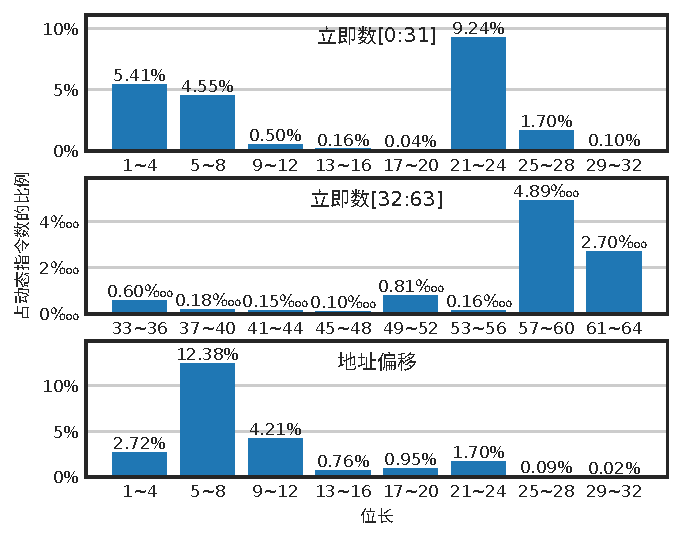
\includegraphics[width=0.8\linewidth]{./plot/immsize_x86.pdf}
  \caption{X86 SPEC CPU 2017 中立即数和地址偏移的分布}
  \label{img:immsize_x86}
\end{figure}

\begin{figure}[h]
  \centering
  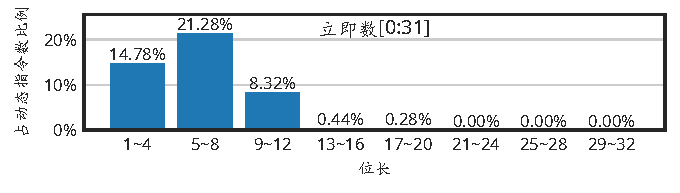
\includegraphics[width=0.8\linewidth]{./plot/immsize_riscv.pdf}
  \caption{RISCV SPEC CPU 2017 中立即数分布}
  \label{img:immsize_riscv}
\end{figure}

因此参考微码缓存的设计思路,我们将短的立即数直接编码在操作数中,长的立即数存储在微码缓存行的立即数区域。
由于指令编码空间有限,并且出于简洁性的考虑,我们只把4比特以下的立即数编码在操作数中,更长的立即数存储在立即数区域,
前者称为\textbf{直接立即数},后者称为\textbf{间接立即数},用5比特的操作数(opr)最高位来区分;
如果为0,表示直接立即数,把短立即数直接编码在操作数中;如果为1,表示间接立即数,把长立即数的长度(len)编码在操作数中,
而真正的立即数需要根据立即数的索引到立即数区域中查找。
存储立即数长度(len)是为了支持\textbf{变长立即数},例如0x1ff,需要2字节来存储,而0x1ff00,需要3字节来存储,这样可以根据len来到立即数区域中取出对应长度的立即数,
并不需要每个立即数都使用4字节存储。


\subsection{寄存器}

目前主流指令集都支持的通用寄存器数量不同,例如X86有16个通用寄存器,RISCV和AArch64有32个通用寄存器。
过少的通用寄存器数量会导致寄存器分配困难,会溢出到内存中,增加访存开销;
过多的通用寄存器数量会导致更多的寄存器编码,增加编码空间,因此我们的设计中,只支持32个通用寄存器的编码,通过5比特的操作数(opr)来寻址寄存器。

由于翻译器还需要使用一些临时寄存器,例如用于存储中间结果的寄存器,对于32个通用寄存器可能不够用,因此我们还需要支持\textbf{临时寄存器},
临时寄存器类似于X86的段寄存器或者RISCV的CSR寄存器,只能用于存储临时数据,不能用于通用寄存器的操作。
所以还需要添加一些搬运指令,用于临时寄存器和通用寄存器之间的数据搬运。

对于浮点寄存器,目前主流指令集都是使用单独的浮点寄存器(X87 会使用浮点栈,我们并不支持,目前gcc编译生成的代码也基本不会使用X87),
例如X86 SSE指令集有16个128位的浮点寄存器,
RISCV有32个64位的浮点寄存器。综合考虑,我们的设计中,只支持32个128位宽浮点寄存器的编码,同样通过5比特的操作数(opr)来寻址浮点寄存器。





\section{RISCV指令语义差异}

上节中的融合微码编码设计是支持多种指令集的基础,本节主要介绍RISCV指令和X86指令的语义差异,以及如何通过添加微码指令来支持RISCV指令。

设计一套高效完备的融合微码“指令集”是一个长期的工程,这不是本文研究重点。
为了快速验证微译器的实际效果,同时减少“指令集设计”产生的额外性能影响,
因此目前我们的融合微码是基于原本的Gem5 X86微码上\textbf{扩充}的,
基于这种扩充的方式,所有X86指令都可以直接翻译成一条或者多条融合微码指令,而RISCV指令的翻译则
需要分析RISCV指令和X86指令(X86微码)的语义差异,然后添加新的融合微码指令。

如图\ref{img:TISA},由于X86指令默认符号扩展,而RISCV指令同时支持符号扩展和零扩展,
为了尽可能实现一条RISCV指令翻译成一条融合微码指令,所以需要添加适当的“零扩展”微码指令。

\begin{figure}[!htbp]
  \centering
  \includegraphics[width=0.8\linewidth]{./image/TISA.pdf}
  \caption{指令翻译到融合微码过程,X86 add 和RISCV add 指令都翻译成融合微码add指令,
  而lbu(加载字节并无符合扩展)指令,需要额外添加lbu 微码指令。}
  \label{img:TISA}
\end{figure}



目前已经完成所有的RISCV指令(包括IMAFDC指令集)到融合微码的翻译,完整的翻译表格见附录\ref{app:RISCV}。

\subsection{整数指令}


\subsection{乘除法指令}


\subsection{原子指令}


\subsection{浮点指令}


\subsection{压缩指令}


\begin{itemize}
  \item 整数指令(I): 主要包括移位指令、算数指令、逻辑指令、比较指令、分支指令、访存指令等。大部分复用X86微码,访存指令等需要额外添加新的微码。

  \item 乘除法指令(M):主要包括乘法、除法、取余等指令。大部分复用X86微码。

  \item 原子指令(A):包括原子加法、原子比较等指令。由于目前尚未实现多线程支持,
  原子加法指令被翻译为一条普通load+加法指令+一条store指令。

  \item 浮点指令(F,D):包括单精度浮点F 和双精度浮点D指令。大部分复用X86微码,出于简洁考虑,对于特殊的舍入模式暂未考虑和X86的差异。

  \item 压缩指令(C):为了压缩指令长度,把常用的4字节指令替换为2字节长度的压缩指令。尽可能把翻译得到的微码也编码为2字节。

\end{itemize}

累积统计数目如下:原本X86指令共有数千条,X86微码也有500余条。
为了添加272条RISCV指令,我们并没有简单添加272条微码指令,
而只是添加了41条整数相关指令,10条浮点相关指令,累计添加51条微码指令。





\section{RISCV ABI差异}
%介绍什么是ABI, 从而引出RISCV和X86的ABI差异。而我们的项目需要把RISCV的ABI转换成X86的ABI。
ABI全称为Aplication Binary Interface,是程序和硬件的统一接口,不同指令集的ABI也是不同的,
在二进制翻译系统中需要维护这种差异性,保证程序运行的正确性。
ABI包括内容比较多,其中主要的包括系统调用传参、初始化栈等问题,本节介绍微译器项目是如何处理ABI差异的。


\subsection{系统调用差异}

如表\ref{tab:syscall}所示,X86和RISCV的系统调用号和参数传递方式的差异。
X86的系统调用号存储在rax寄存器中,返回值也存储在rax寄存器中,参数传递方式为rdi, rsi, rdx, r10, r8, r9。
而RISCV的系统调用号存储在a7寄存器中,返回值存储在a0寄存器中,参数传递方式为a0, a1, a2, a3, a4, a5。
因此我们需要在RISCV的二进制翻译器中,将RISCV的系统调用号和参数传递方式转换成X86的系统调用号和参数传递方式。

参数传递的差异可以通过把X86的参数寄存器和RISCV的参数寄存器映射到相同的微码寄存器即可,如表\ref{tab:reg_map}所示,
所有的黄色寄存器就是6个参数传递寄存器。系统调用号差异同理也可解决。



\begin{table}[h]
    \centering
    \begin{adjustbox}{width=\textwidth}
      \begin{tabular}{llllllllll}
      \rowcolor[HTML]{FFCC67} 
      \cellcolor[HTML]{FBE5D6}指令集 & \cellcolor[HTML]{FBE5D6}系统调用号 & \cellcolor[HTML]{FBE5D6}返回值 & 参数1 & 参数2 & 参数3 & 参数4 & 参数5 & 参数6 & 其他参数 \\
      X86                         & rax                           & rax                         & rdi & rsi & rdx & r10 & r8  & r9  & 栈传递  \\
      RISCV                       & a7                            & a0                          & a0  & a1  & a2  & a3  & a4  & a5  & 栈传递 
      \end{tabular}
    \end{adjustbox}
    \caption{X86和RISCV的系统调用号和参数传递方式的差异。}
    \label{tab:syscall}
  \end{table}
  

\subsection{寄存器映射}

寄存器映射一直是二进制翻译中一个重要的研究课题。
如表\ref{tab:reg_map}所示,展示了X86和RISCV映射到微码的的寄存器映射表。
对于X86寄存器映射到微码寄存器较为容易,因为X86只有16个通用整数寄存器,而微码我们定义了32个通用寄存器,
所以只需要把X86寄存器固定映射到前16个通用寄存器即可,还可以把一些常用的寄存器
(例如AH,BH等子寄存器和段寄存器)映射到后面的寄存器中,还可用一些寄存器作为临时寄存器供二进制翻译器使用。

但是对于RISCV映射到微码方案,由于RISCV本身就有32个通用寄存器,固定映射到32个微码寄存器后,
就没有额外的临时寄存器供二进制翻译器使用了。对于微译器项目,得益于软硬件协同设计的基本原则,
我们额外添加了两个微码寄存器作为临时寄存器,
这两个寄存器只对二进制翻译器可见,不对RISCV应用程序可见,类似于X86“段寄存器”,属于特殊寄存器。



\begin{table}[]
  \centering
  \caption{
    X86和RISCV的寄存器映射表。
  }
  \label{tab:reg_map}
  \begin{adjustbox}{width=\textwidth}
  \begin{tabular}{|
    >{\columncolor[HTML]{FFCCC9}}l |l|l|
    >{\columncolor[HTML]{FFCCC9}}l |
    >{\columncolor[HTML]{FFFFFF}}l |
    >{\columncolor[HTML]{FFFFFF}}l |
    >{\columncolor[HTML]{FFCCC9}}l |
    >{\columncolor[HTML]{FFFFFF}}l |
    >{\columncolor[HTML]{FFFFFF}}l |
    >{\columncolor[HTML]{FFCCC9}}l |
    >{\columncolor[HTML]{FFFFFF}}l |
    >{\columncolor[HTML]{FFFFFF}}l |}
    \hline
    \cellcolor[HTML]{FBE5D6}微码 & \cellcolor[HTML]{FBE5D6}X86 & \cellcolor[HTML]{FBE5D6}RISCV & \cellcolor[HTML]{FBE5D6}微码 & \cellcolor[HTML]{FBE5D6}X86 & \cellcolor[HTML]{FBE5D6}RISCV & \cellcolor[HTML]{FBE5D6}微码 & \cellcolor[HTML]{FBE5D6}X86 & \cellcolor[HTML]{FBE5D6}RISCV & \cellcolor[HTML]{FBE5D6}微码 & \cellcolor[HTML]{FBE5D6}X86 & \cellcolor[HTML]{FBE5D6}RISCV \\ \hline
    0                          & \cellcolor[HTML]{FFFC9E}RAX & \cellcolor[HTML]{FFFC9E}A7    & 8                          & \cellcolor[HTML]{FFFC9E}R8  & \cellcolor[HTML]{FFFC9E}A4    & 16                         & T0                          & Zero                          & 24                         & CH                          & S8                            \\ \hline
    1                          & \cellcolor[HTML]{FFFFFF}RCX & \cellcolor[HTML]{FFFFFF}TP    & 9                          & \cellcolor[HTML]{FFFC9E}R9  & \cellcolor[HTML]{FFFC9E}A5    & 17                         & T1                          & RA                            & 25                         & DH                          & S9                            \\ \hline
    2                          & \cellcolor[HTML]{FFFC9E}RDX & \cellcolor[HTML]{FFFC9E}A2    & 10                         & \cellcolor[HTML]{FFFC9E}R10 & \cellcolor[HTML]{FFFC9E}A3    & 18                         & T2                          & S2                            & 26                         & ES                          & S10                           \\ \hline
    3                          & \cellcolor[HTML]{FFFFFF}RBX & \cellcolor[HTML]{FFFFFF}GP    & 11                         & R11                         & A6                            & 19                         & T3                          & S3                            & 27                         & CS                          & S11                           \\ \hline
    4                          & \cellcolor[HTML]{FFFFFF}RSP & \cellcolor[HTML]{FFFFFF}SP    & 12                         & R12                         & T1                            & 20                         & T4                          & S4                            & 28                         & SS                          & T3                            \\ \hline
    5                          & \cellcolor[HTML]{FFFFFF}RBP & \cellcolor[HTML]{FFFFFF}T0    & 13                         & R13                         & T2                            & 21                         & T5                          & S5                            & 29                         & DS                          & T4                            \\ \hline
    6                          & \cellcolor[HTML]{FFFC9E}RSI & \cellcolor[HTML]{FFFC9E}A1    & 14                         & R14                         & S0                            & 22                         & AH                          & S6                            & 30                         & FS                          & T5                            \\ \hline
    7                          & \cellcolor[HTML]{FFFC9E}RDI & \cellcolor[HTML]{FFFC9E}A0    & 15                         & R15                         & S1                            & 23                         & BH                          & S7                            & 31                         & GS                          & T6                            \\ \hline
  \end{tabular}
  \end{adjustbox}
\end{table}

% \subsection{栈的初始化}
% 由于我们目前关注于用户态二进制翻译器,不太涉及系统态指令的翻译和处理操作系统等概念,
% 但是当加载运行不同指令集的程序时,在libc库眼中,操作系统已经准备好了这个程序的初始化栈等信息,例如argc,argv参数、
% 环境变量指针等,对于X86和RISCV程序,这个初始化栈是不同的,需要不同的处理